% ============================================================================
% 附录 AJ：加料与排灰——燃料怎么进去，灰怎么出来
% 数值唯一来源：tools/calc/appAJ_calc.py -> tools/calc/appAJ_calc.txt（只 print，不写文件）
% 单位写法：数字与单位都进数学模式（避免中文字符进数学字体）；温度用 eV，质量用 kg，
%          流量用 Pa m^3/s 与 mbar L/s 并列，粒子数一律给 s^-1。
% 工作点：n_e = 1e20 m^-3、T_e = 9.194 keV、B = 5.3 T、a = 2.0 m、R = 6.2 m、
%         V = 832.2 m^3、P_fus = 556.5 MW、P_alpha = 111.3 MW（与附录 M/S/U/V/W/X/Y/Z/AD/AI 同点）。
%         氚质量取附录 Z 的 m_T = 3.0160492 u，库存上限取附录 Z 的 2.0 kg。
% 版权口径：只借鉴结论、公式形式与题型；正文文字、数值、表格自拟并独立复算。
%          离线环境无法核验 DOI，故只给书名/作者/年份/卷期页。
% 分工：附录 AD 讲边界台基与 ELM，本附录只讲「粒子怎么进、灰怎么出」；
%      附录 Z 讲氚循环与自持的工程账，本附录补上它前面的加料物理与库存来源。
% ============================================================================

\section{粒子平衡：加进去的粒子有多少被烧掉}
\label{sec:app-aj-balance}

聚变堆的第一个不确定数是「要往里灌多少燃料」。这个数不能拍脑袋，
它由三笔账决定：烧掉多少、漏掉多少、回来多少。

先算烧掉多少。聚变功率 $P_{\mathrm{fus}} = 556.5\ \mathrm{MW}$ 是宏观量，
每次 D-T 反应放出的总能量是 $17.6\ \mathrm{MeV}$，所以反应率是

\begin{equation}
R_{\mathrm{fus}} = \frac{P_{\mathrm{fus}}}{E_{\mathrm{fus}}}
= \frac{556.5\times10^{6}}{17.6\times1.602176634\times10^{-13}}
= 1.97352\times10^{20}\ \mathrm{s^{-1}},
\label{eq:app-aj-rfus}
\end{equation}

每次反应吃掉一个氘核和一个氚核，所以离子的燃烧消耗率是它的两倍：
$3.94705\times10^{20}\ \mathrm{s^{-1}}$。换成质量，氚的燃耗是

\begin{equation}
\dot m_T = R_{\mathrm{fus}}\,m_T = 1.97352\times10^{20}\times5.00827\times10^{-27}
= 9.88481\times10^{-7}\ \mathrm{kg\,s^{-1}} = 31.1913\ \text{kg/年},
\label{eq:app-aj-burn}
\end{equation}

这正是附录 Z 里那个 $31.19\ \text{kg/年}$——同一个工作点、同一套常数，两条路必须对上。

再看漏掉多少。粒子约束时间 $\tau_p = 2.5\ \mathrm{s}$（声明值）意味着总电子数
$N_e = n_eV = 8.322\times10^{22}$ 每隔几秒就换一遍：

\begin{equation}
\frac{N_e}{\tau_p} = \frac{8.322\times10^{22}}{2.5}
= 3.3288\times10^{22}\ \mathrm{s^{-1}}.
\label{eq:app-aj-loss}
\end{equation}

把燃烧和输运加起来，总损失是 $3.36827\times10^{22}\ \mathrm{s^{-1}}$——
注意 \textbf{输运损失比燃烧大 84 倍}，这就是加料问题的全部难点。

最后看回来多少。打到壁上的粒子有 $R = 0.95$（声明值）会以中性粒子的形式
回到等离子体里，真正需要从外部补的只有剩下那一点，再加上烧掉的那一份：

\begin{equation}
S_{\mathrm{ext}} = (1-R)\,\frac{N_e}{\tau_p} + 2R_{\mathrm{fus}}
= 0.05\times3.3288\times10^{22} + 3.94705\times10^{20}
= 2.0591\times10^{21}\ \mathrm{s^{-1}}.
\label{eq:app-aj-recycle}
\end{equation}

这个数只有输运损失的 $6.18573\%$，却是燃烧量的 $5.21683$ 倍。
于是得到本附录最该记住的一句话：

\begin{equation}
f_{\mathrm{burn}} = \frac{2R_{\mathrm{fus}}}{S_{\mathrm{ext}}}
= \frac{3.94705\times10^{20}}{2.0591\times10^{21}} = 19.1687\%.
\label{eq:app-aj-burnfrac}
\end{equation}

「净加料里有 $19\%$ 被烧掉」听起来还不错。但这是\textbf{净}加料：
真正从阀门和弹丸枪注进去的粒子还要乘上加料效率，而气体加料的效率只有 $10\%$ 量级。
把这一层算进去，注进去的粒子只有 $1.91687\%$ 被烧掉——\textbf{其余 $98\%$ 都被抽走了}。

\begin{table}[htbp]
\centering
\small
\begin{tabular}{p{3.2cm}p{3.2cm}p{3.1cm}p{3.8cm}}
\toprule
量 & 表达式 & 数值 & 说明 \\
\midrule
电子总数 $N_e$ & $n_eV$ & $8.322\times10^{22}$ & 工作点存量 \\
聚变反应率 & $P_{\mathrm{fus}}/E_{\mathrm{fus}}$ & $1.97352\times10^{20}\ \mathrm{s^{-1}}$ & 由功率反推 \\
燃烧消耗率 & $2R_{\mathrm{fus}}$ & $3.94705\times10^{20}\ \mathrm{s^{-1}}$ & D 与 T 各一份 \\
氚燃耗 & $R_{\mathrm{fus}}m_T$ & $31.1913\ \text{kg/年}$ & 与附录 Z 同口径 \\
输运损失 & $N_e/\tau_p$ & $3.3288\times10^{22}\ \mathrm{s^{-1}}$ & 比燃烧大 84 倍 \\
外部加料需求 & $(1-R)N_e/\tau_p + 2R_{\mathrm{fus}}$ & $2.0591\times10^{21}\ \mathrm{s^{-1}}$ & 再循环帮了大忙 \\
净加料燃耗份额 & $2R_{\mathrm{fus}}/S_{\mathrm{ext}}$ & $19.1687\%$ & 注进去只有 $1.91687\%$ \\
\bottomrule
\end{tabular}
\caption{工作点的粒子账。三笔账的顺序不能颠倒：先算燃烧，再算输运，最后才谈加料。}
\label{tab:app-aj-balance}
\end{table}

\begin{tip}{加料量不是燃烧量}{tip-app-aj-balance}
「聚变堆每秒烧掉多少燃料」和「每秒要灌进多少燃料」是两个数：本例净加料是燃烧量的
$5.21683$ 倍，按注气量算则是 $52.1683$ 倍。凡是看到「加料量」三个字，
先问它是净加料还是注气量。加料系统的规模由后者决定，氚厂的规模由燃耗决定，
两者差一个到两个量级。
\end{tip}

{\footnotesize
\textbf{出处：}粒子平衡与再循环的处理参照 Wesson \emph{Tokamaks}（第 4 版，2011，第 1、6 章）。
Freidberg \emph{Plasma Physics and Fusion Energy}（2007，第 13--14 章）与
ITER Physics Basis（1999，\emph{Nucl. Fusion} \textbf{39}, 2137，第 2 章）。
$17.6\ \mathrm{MeV}$ 与氚质量取与附录 Z 相同的口径。
}

\section{气体加料与弹丸加料：效率差在哪}
\label{sec:app-aj-fuelling}

把 $2.0591\times10^{21}\ \mathrm{s^{-1}}$ 的净需求交给两种加料方式，得到完全不同的注入量。

气体加料靠的是从阀门喷出的中性气体，它在边界就被电离，
大部分沿磁力线直接流向偏滤器，能进芯部的只有 $10\%$ 量级。要凑够净需求，注气量是

\begin{equation}
S_{\mathrm{gas}} = \frac{S_{\mathrm{ext}}}{\eta_{\mathrm{gas}}}
= \frac{2.0591\times10^{21}}{0.10} = 2.0591\times10^{22}\ \mathrm{s^{-1}},
\label{eq:app-aj-gasinj}
\end{equation}

换算成工程上惯用的流量（$300\ \mathrm{K}$ 的 $\mathrm{D_2}$，每个分子给两个原子）：

\begin{equation}
\begin{aligned}
Q_{\mathrm{gas}} &= \frac{S_{\mathrm{gas}}}{2}\,k_BT
= \frac{2.0591\times10^{22}}{2}\times1.380649\times10^{-23}\times300 \\
&= 42.6435\ \mathrm{Pa\,m^{3}\,s^{-1}} = 426.435\ \mathrm{mbar\,L\,s^{-1}}.
\end{aligned}
\label{eq:app-aj-gasflow}
\end{equation}

弹丸加料则把燃料做成 $1.5\ \mathrm{mm}$ 的冰丸（$\rho = 255\ \mathrm{kg\,m^{-3}}$），
以 $300\ \mathrm{m\,s^{-1}}$ 打进去，效率可到 $60\%$ 量级。注入量降为
$3.43184\times10^{21}\ \mathrm{s^{-1}}$，质量流率

\begin{equation}
\dot m_{\mathrm{pel}} = \frac{S_{\mathrm{ext}}}{2\eta_{\mathrm{pel}}}\,m_i
= \frac{2.0591\times10^{21}}{2\times0.60}\times4.15135\times10^{-27}
= 7.12338\times10^{-6}\ \mathrm{kg\,s^{-1}} = 7.12338\ \mathrm{mg\,s^{-1}},
\label{eq:app-aj-pelletmass}
\end{equation}

即 $615.46\ \mathrm{g/day}$、$224.797\ \text{kg/年}$。
\textbf{同样的净需求，注气量是弹丸量的 6 倍}——这正是弹丸加料存在的理由：
不是它更便宜，是它把粒子放到了更里面。

\begin{table}[htbp]
\centering
\small
\begin{tabular}{p{2.8cm}p{3.2cm}p{3.2cm}p{4.2cm}}
\toprule
方式 & 加料效率（声明） & 注入量 & 工程口径 \\
\midrule
气体加料 & $10\%$ & $2.0591\times10^{22}\ \mathrm{s^{-1}}$ & $42.6435\ \mathrm{Pa\,m^{3}\,s^{-1}}$（$426.435\ \mathrm{mbar\,L\,s^{-1}}$） \\
弹丸加料 & $60\%$ & $3.43184\times10^{21}\ \mathrm{s^{-1}}$ & $7.12338\ \mathrm{mg\,s^{-1}}$（$615.46\ \mathrm{g/day}$） \\
超声分子束 & 介于两者之间 & 与气体同量级 & 靠定向高速中性流提高穿透 \\
紧凑环注入 & 芯部加料 & 与弹丸同量级 & 把等离子体团整体注入 \\
\bottomrule
\end{tabular}
\caption{四种加料方式。效率是\textbf{声明值}，只用于量级比较；真实效率取决于穿透深度与边界条件。}
\label{tab:app-aj-fuelling}
\end{table}

\begin{tip}{效率低不是浪费，是物理}{tip-app-aj-efficiency}
气体加料效率只有 $10\%$ 不是「技术不行」，而是中性粒子在边界就被电离、
电离之后只能沿磁力线走的必然结果。想提高效率，办法不是加大阀门，而是
\textbf{把粒子送到电离之前就已经很深的地方}——弹丸、超声分子束、紧凑环都是这个思路。
\end{tip}

{\footnotesize
\textbf{出处：}弹丸加料的综述与效率区间参照 Milora 等（1995，\emph{Nucl. Fusion} \textbf{35}, 657）。
边缘再循环与加料效率的处理参照 Stangeby \emph{The Plasma Boundary of Magnetic Fusion Devices}
（2000，第 4 章）与 Loarte 等（2007，\emph{Nucl. Fusion} \textbf{47}, S203，ITER 物理基础第 4 章）。
}

\begin{figure}[htbp]
\centering
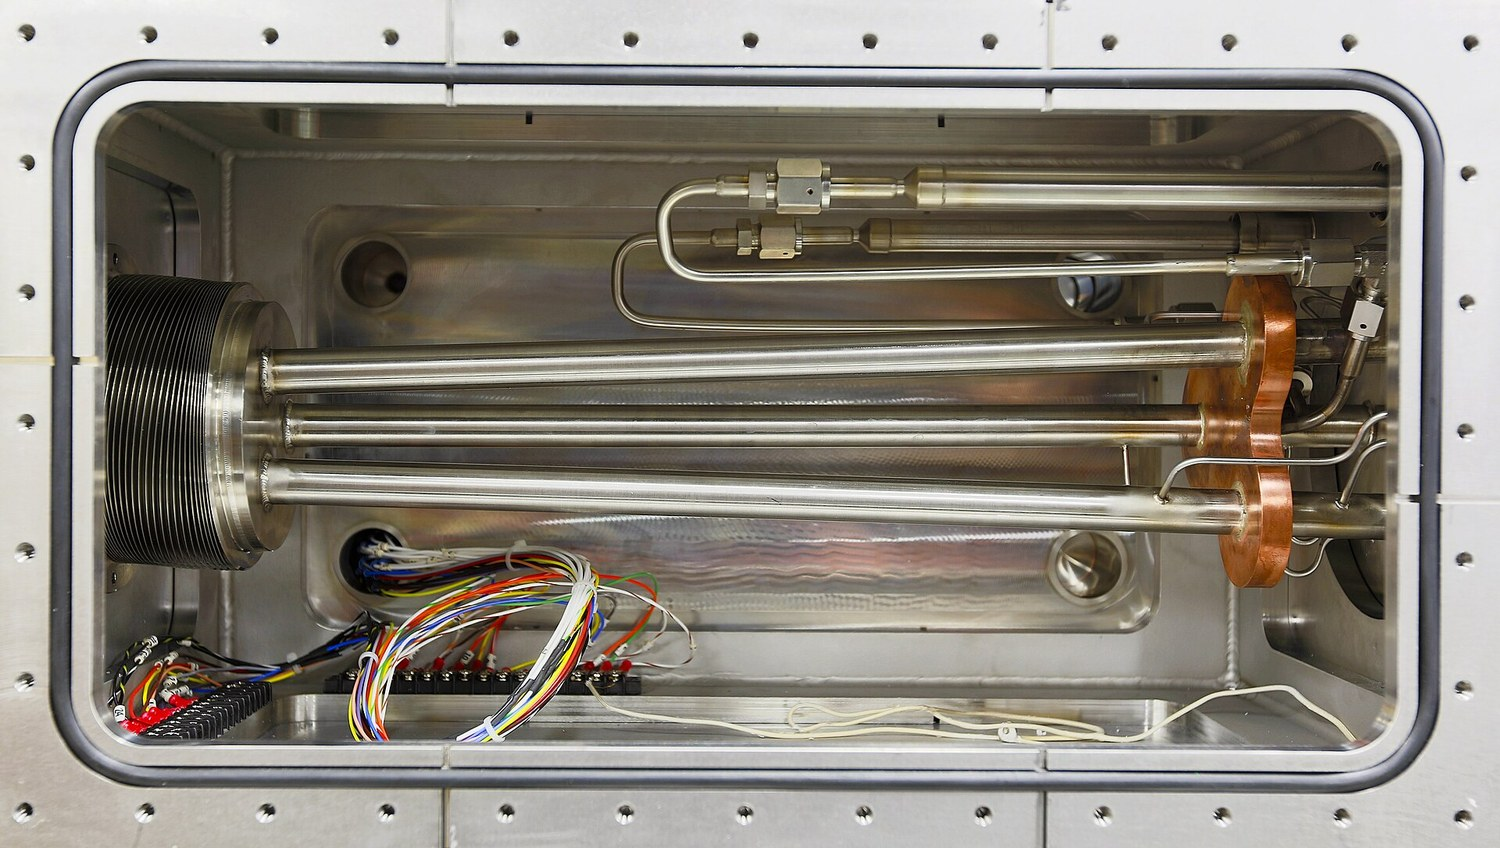
\includegraphics[width=0.72\textwidth]{../figures/pellet_injector.jpg}
\caption{弹丸注入器：燃料以固体弹丸的形式进堆。弹丸加料之所以效率高，是因为它把燃料直接送到芯部，而不是靠边界再往里扩散；本节算的烧蚀与穿透深度，决定了这颗弹丸能走多深——图中的三条炮管正是为了在一次注入里给出不同深度与不同粒径的组合。}
\label{fig:photo-appaj}
\figsource{Oak Ridge National Laboratory，CC BY 2.0（Wikimedia Commons）}
\end{figure}

\section{弹丸烧蚀与穿透：中性气体屏蔽}
\label{sec:app-aj-pellet}

弹丸为什么能钻进等离子体？因为它一路上被自己蒸发出来的气体包住。
这层中性气体把等离子体的热流挡在外面（中性气体屏蔽，NGS），
烧蚀速度因此由「热流穿过气盾的传导」决定，而不是由表面温度决定。
标准标度是：半径损失率 $\dot r \propto r^{-2/3}$，于是烧蚀时间

\begin{equation}
\tau_{\mathrm{abl}} \propto r_p^{5/3},
\qquad
L_{\mathrm{pen}} = v_p\,\tau_{\mathrm{abl}},
\label{eq:app-aj-abl}
\end{equation}

工作点取 $\tau_{\mathrm{abl}} = 0.4\ \mathrm{ms}$（声明值，$r_p = 1.5\ \mathrm{mm}$、
$n_e = 10^{20}\ \mathrm{m^{-3}}$），弹丸速度 $300\ \mathrm{m\,s^{-1}}$，则

\begin{equation}
L_{\mathrm{pen}} = 300\times4.0\times10^{-4} = 0.12\ \mathrm{m} = 12\ \mathrm{cm},
\label{eq:app-aj-pen}
\end{equation}

只有小半径 $a = 2.0\ \mathrm{m}$ 的 $6\%$。换句话说，$1.5\ \mathrm{mm}$ 的弹丸
\textbf{在边缘就烧完了}，它的粒子主要沉积在最外面十几厘米——加料效率上不去的原因就在这里。

\begin{equation}
m_p = \frac{4}{3}\pi r_p^{3}\rho_{\mathrm{ice}}
= \frac{4}{3}\pi(1.5\times10^{-3})^{3}\times255
= 3.60498\times10^{-6}\ \mathrm{kg} = 3.60498\ \mathrm{mg},
\label{eq:app-aj-pelletmass2}
\end{equation}

其中氚占 $2.16299\ \mathrm{mg}$，含 $8.68387\times10^{20}$ 个 D-T 原子
（与附录 AD 的「$10^{21}$ 个原子 $= 4.18155\ \mathrm{mg}$」同一口径）。
按 $7.12338\ \mathrm{mg\,s^{-1}}$ 的流率，弹丸频率是

\begin{equation}
f_p = \frac{\dot m_{\mathrm{pel}}}{m_p}
= \frac{7.12338\times10^{-6}}{3.60498\times10^{-6}} = 1.97599\ \mathrm{Hz},
\label{eq:app-aj-pelletfreq}
\end{equation}

即每 $0.506077\ \mathrm{s}$ 一发。这个周期后面讲密度控制时还要用。

\begin{table}[htbp]
\centering
\small
\begin{tabular}{p{2.6cm}p{2.6cm}p{2.6cm}p{2.6cm}p{3.4cm}}
\toprule
$r_p$ & 质量 & $\tau_{\mathrm{abl}}$ & $L_{\mathrm{pen}}$ & 说明 \\
\midrule
$1.5\ \mathrm{mm}$ & $3.60498\ \mathrm{mg}$ & $0.4\ \mathrm{ms}$ & $0.12\ \mathrm{m}$ & 占 $a$ 的 $6\%$，边缘加料 \\
$2\ \mathrm{mm}$ & $8.54513\ \mathrm{mg}$ & $0.646087\ \mathrm{ms}$ & $0.193826\ \mathrm{m}$ & 仍在外半区 \\
$3\ \mathrm{mm}$ & $28.8398\ \mathrm{mg}$ & $1.26992\ \mathrm{ms}$ & $0.380976\ \mathrm{m}$ & 占 $a$ 的 $19.0488\%$ \\
$3\ \mathrm{mm}$（$1000\ \mathrm{m\,s^{-1}}$） & $28.8398\ \mathrm{mg}$ & $1.26992\ \mathrm{ms}$ & $1.26992\ \mathrm{m}$ & $L/a = 0.63496$，够到芯部 \\
\bottomrule
\end{tabular}
\caption{弹丸穿透的标度扫描。$\tau_{\mathrm{abl}} \propto r_p^{5/3}$、$L_{\mathrm{pen}} \propto v_pr_p^{5/3}$，
所以\textbf{加大弹丸比提速更有效}（体积涨三次方，烧蚀时间只涨 $5/3$ 次方）。}
\label{tab:app-aj-pellet}
\end{table}

要让弹丸打到 $a/2 = 1\ \mathrm{m}$（芯部加料的最低要求），
$r_p = 1.5\ \mathrm{mm}$ 需要 $v_p \ge 2500\ \mathrm{m\,s^{-1}}$；
把半径加大到 $3\ \mathrm{mm}$，速度只需 $787.451\ \mathrm{m\,s^{-1}}$。
这正是离心加速弹丸枪把速度做到公里每秒量级的原因。

\begin{tip}{弹丸是被自己的气体盾牌挡住的}{tip-app-aj-ngs}
中性气体屏蔽听起来像「保护层」，其实是双刃剑：它挡住了热流（所以弹丸能活到那么深），
也把弹丸的蒸发限制在表层（所以烧蚀长度正比于 $r^{5/3}$ 而不是 $r$）。
穿透深度的物理全部藏在这层气盾的传导里，不在弹丸材料上。
\end{tip}

{\footnotesize
\textbf{出处：}中性气体屏蔽与烧蚀标度参照 Parks \& Turnbull（1978，\emph{Phys. Fluids} \textbf{21}, 1735）。
弹丸参数区间与加料效率参照 Milora 等（1995，\emph{Nucl. Fusion} \textbf{35}, 657）。
几何口径与附录 AD 的弹丸原子数保持一致。
}

\section{氦灰：稀释与排出条件}
\label{sec:app-aj-ash}

D-T 反应每放出一个中子，就留下一个氦核。氦是「灰」不是「杂质」：
它带电、被磁场约束、又几乎不参与聚变——留在芯部只会稀释燃料。

稳态氦密度由产生率和停留时间决定。取 $\tau_{\mathrm{He}}^{*} = 5\tau_E = 18.5\ \mathrm{s}$（声明值）：

\begin{equation}
n_{\mathrm{He}} = \frac{R_{\mathrm{fus}}\tau_{\mathrm{He}}^{*}}{V}
= \frac{1.97352\times10^{20}\times18.5}{832.2}
= 4.38719\times10^{18}\ \mathrm{m^{-3}},
\qquad
\frac{n_{\mathrm{He}}}{n_e} = 4.38719\%.
\label{eq:app-aj-ashdens}
\end{equation}

氦是双电荷，每两个电子被一个氦核占住，所以燃料离子密度只剩

\begin{equation}
n_{\mathrm{fuel}} = n_e - 2n_{\mathrm{He}} = 9.12256\times10^{19}\ \mathrm{m^{-3}}
= 91.2256\%\,n_e .
\label{eq:app-aj-dilute}
\end{equation}

聚变功率正比于 $n_Dn_T \propto n_{\mathrm{fuel}}^{2}$，于是一路稀释下来：

\begin{equation}
P_{\mathrm{fus}} \to 556.5\times(0.912256)^{2} = 463.126\ \mathrm{MW}
= 83.2211\%\,P_{\mathrm{fus}} .
\label{eq:app-aj-ashreq}
\end{equation}

\textbf{$4.4\%$ 的灰吃掉 $16.8\%$ 的功率}——这就是灰必须排掉的全部理由。
反过来说，若要把灰压到 $5\%$ 以内，停留时间必须满足

\begin{equation}
\tau_{\mathrm{He}}^{*} \le \frac{0.05\,n_eV}{R_{\mathrm{fus}}}
= \frac{0.05\times10^{20}\times832.2}{1.97352\times10^{20}} = 21.0841\ \mathrm{s}
\quad\Longrightarrow\quad
\frac{\tau_{\mathrm{He}}^{*}}{\tau_E} \le 5.69841 .
\label{eq:app-aj-ashreq2}
\end{equation}

「灰的停留时间不超过能量约束时间的五到六倍」是聚变堆的一条硬指标，
它和 $\tau_E$ 一起决定了偏滤器的抽气设计。

\begin{table}[htbp]
\centering
\small
\begin{tabular}{p{3.2cm}p{3.0cm}p{3.0cm}p{3.6cm}}
\toprule
量 & 表达式 & 数值 & 说明 \\
\midrule
氦产生率 & $R_{\mathrm{fus}}$ & $1.97352\times10^{20}\ \mathrm{s^{-1}}$ & 每个反应一个 \\
停留时间 & $5\tau_E$ & $18.5\ \mathrm{s}$ & 声明口径 \\
稳态氦密度 & $R_{\mathrm{fus}}\tau_{\mathrm{He}}^{*}/V$ & $4.38719\times10^{18}\ \mathrm{m^{-3}}$ & 即 $4.38719\%\,n_e$ \\
燃料离子密度 & $n_e - 2n_{\mathrm{He}}$ & $9.12256\times10^{19}\ \mathrm{m^{-3}}$ & $91.2256\%\,n_e$ \\
稀释后功率 & $\propto n_{\mathrm{fuel}}^{2}$ & $463.126\ \mathrm{MW}$ & $83.2211\%$ \\
排出条件 & $\tau_{\mathrm{He}}^{*}/\tau_E \le 5.69841$ & $21.0841\ \mathrm{s}$ & 压到 $5\%$ 以内 \\
偏滤器处氦密度 & 富集 $5$ 倍（声明） & $2.5\times10^{19}\ \mathrm{m^{-3}}$ & 富集是抽气的必要条件 \\
\bottomrule
\end{tabular}
\caption{氦灰的三笔账：产生、稀释、排出条件。富集因子是声明值，只作量级说明。}
\label{tab:app-aj-ash}
\end{table}

灰的存在也能看见：氦的谱线（如 He II $468.57\ \mathrm{nm}$，见附录 AH）
是边界氦密度的常规诊断，只是从谱线到芯部灰份额要经过输运模型的反演。

\begin{tip}{灰不是杂质，是产物}{tip-app-aj-ash}
杂质可以靠「少产生」来解决，灰不行——它的产生率被聚变功率锁死。
所以氦灰问题从来不是「如何不产生」，而是「如何在它稀释燃料之前把它送出去」。
这也是为什么偏滤器设计对聚变堆是生死问题。
\end{tip}

{\footnotesize
\textbf{出处：}功率与粒子控制（含氦灰排出条件）参照 Loarte 等（2007，\emph{Nucl. Fusion} \textbf{47}, S203）
与 ITER Physics Basis（1999，\emph{Nucl. Fusion} \textbf{39}, 2137，第 4 章）。
反应率与稀释的处理参照 Bosch \& Hale（1992，\emph{Nucl. Fusion} \textbf{32}, 611）与 Wesson
\emph{Tokamaks}（第 4 版，2011，第 6 章）。
氦谱线见附录 AH。本节凡标出数字的量都由
\texttt{tools/\allowbreak{}calc/\allowbreak{}appAJ\_calc.py} 复算。
}

\section{抽气与氚存量：为什么瓶颈不在泵上}
\label{sec:app-aj-pumping}

偏滤器的抽气能力常被误认为是排灰的瓶颈。算一下就清楚了：
偏滤器中性气体压力 $5\ \mathrm{Pa}$（声明）、抽气速率 $100\ \mathrm{m^{3}\,s^{-1}}$（声明）、
气体温度 $300\ \mathrm{K}$，则粒子排出率是

\begin{equation}
Q_{\mathrm{pump}} = \frac{P_{\mathrm{div}}S_{\mathrm{pump}}}{k_BT}
= \frac{5\times100}{1.380649\times10^{-23}\times300}
= 1.20716\times10^{23}\ \mathrm{s^{-1}},
\label{eq:app-aj-pumpq}
\end{equation}

是氦产生率的 $611.679$ 倍。换句话说，抽走的气体里只要

\begin{equation}
\frac{R_{\mathrm{fus}}}{Q_{\mathrm{pump}}} = \frac{1.97352\times10^{20}}{1.20716\times10^{23}}
= 0.163485\%
\label{eq:app-aj-hefrac}
\end{equation}

是氦，就足以把灰排干净。\textbf{瓶颈从来不是泵，是把灰从芯部搬到偏滤器的那段输运}——
这正是 $\tau_{\mathrm{He}}^{*}/\tau_E$ 这个指标的意义。

比排灰更麻烦的是氚存量。加料流里的氚是

\begin{equation}
\dot m_T^{\mathrm{fuel}} = \frac{S_{\mathrm{ext}}}{2}m_T
= \frac{2.0591\times10^{21}}{2}\times5.00827\times10^{-27}
= 5.15627\times10^{-6}\ \mathrm{kg\,s^{-1}} = 162.72\ \text{kg/年},
\label{eq:app-aj-inventory}
\end{equation}

是燃耗（$31.1913\ \text{kg/年}$）的 $5.21683$ 倍——\textbf{氚循环要处理的量永远是燃耗的几倍}，
因为大部分氚只是路过。若其中 $1\%$（声明）滞留在壁与灰尘里：

\begin{equation}
\dot m_T^{\mathrm{ret}} = 0.01\times162.72 = 1.6272\ \text{kg/年}
\quad\Longrightarrow\quad
t_{\mathrm{lim}} = \frac{2.0\ \mathrm{kg}}{1.6272\ \text{kg/年}} = 1.22911\ \text{年},
\label{eq:app-aj-inventory2}
\end{equation}

不到 $15$ 个月就到库存上限（$2.0\ \mathrm{kg}$，与附录 Z 同口径）。
把滞留与衰变（$0.112524\ \text{kg/年}$）都算进去，氚自持的下限从附录 Z 的 $1.0036$ 抬到

\begin{equation}
\mathrm{TBR}_{\mathrm{req}} = \frac{31.1913 + 1.6272 + 0.112524}{31.1913} = 1.05578 .
\label{eq:app-aj-tbr}
\end{equation}

\begin{table}[htbp]
\centering
\small
\begin{tabular}{p{3.4cm}p{3.2cm}p{3.0cm}p{3.2cm}}
\toprule
量 & 表达式 & 数值 & 说明 \\
\midrule
抽气排出率 & $PS/k_BT$ & $1.20716\times10^{23}\ \mathrm{s^{-1}}$ & 是氦产生率的 $611.679$ 倍 \\
需要的氦份额 & $R_{\mathrm{fus}}/Q_{\mathrm{pump}}$ & $0.163485\%$ & 泵不是瓶颈 \\
加料氚流 & $S_{\mathrm{ext}}m_T/2$ & $162.72\ \text{kg/年}$ & 燃耗的 $5.21683$ 倍 \\
年滞留 & $1\%$ 的加料氚流 & $1.6272\ \text{kg/年}$ & 声明份额 \\
到库存上限 & $2.0\ \mathrm{kg}/\dot m_T^{\mathrm{ret}}$ & $1.22911\ \text{年}$ & $14.7493$ 个月 \\
衰变损失 & $\ln 2\,M/T_{1/2}$ & $0.112524\ \text{kg/年}$ & 库存 $2.0\ \mathrm{kg}$ \\
自持下限 & 燃耗$+$滞留$+$衰变 & $1.05578$ & 附录 Z 只算衰变是 $1.0036$ \\
\bottomrule
\end{tabular}
\caption{抽气与氚存量。同样的抽气能力，决定库存增长速度的是滞留份额，不是泵速。}
\label{tab:app-aj-pumping}
\end{table}

\begin{tip}{瓶颈不在泵上}{tip-app-aj-pump}
把 $1.20716\times10^{23}\ \mathrm{s^{-1}}$ 的抽气能力与 $1.97352\times10^{20}\ \mathrm{s^{-1}}$
的产灰率放在一起，就知道偏滤器设计真正要保证的是\textbf{把氦送到偏滤器并让它中性化}，
而不是把泵做大。反过来，氚存量问题也提醒：真正需要盯住的是「滞留份额」这个百分比。
\end{tip}

{\footnotesize
\textbf{出处：}偏滤器抽气与再循环的处理参照 Stangeby（2000，第 8 章）与 Loarte 等（2007）。
氚滞留与共沉积的综述参照 Causey（2002，\emph{J. Nucl. Mater.} \textbf{300}, 91）。
氚库存、半衰期与自持口径与附录 Z 一致。本节凡标出数字的量都由
\texttt{tools/\allowbreak{}calc/\allowbreak{}appAJ\_calc.py} 复算。
}

\section{密度控制：反馈回路的带宽}
\label{sec:app-aj-control}

前面五节都是「稳态账」，但装置真正要控制的量是密度随时间的轨迹。
工作点的密度离密度极限有多远？用 Greenwald 经验极限，取等离子体电流
$I_p = 11.0844\ \mathrm{MA}$（与附录 AG 的 $q_{95} = 3$ 工作点同点）：

\begin{equation}
n_G = \frac{I_p}{\pi a^{2}}
= \frac{11.0844\times10^{6}}{\pi\times2.0^{2}}
= 8.82069\times10^{19}\ \mathrm{m^{-3}},
\qquad
\frac{n_e}{n_G} = 1.1337 .
\label{eq:app-aj-greenwald}
\end{equation}

注意这个比值大于 $1$：工作点\textbf{略高于}经验极限，
这是聚变堆设计里必须靠加料剖面与边界条件去处理的问题（附录 AD 与 AG 都讨论过）。

再看响应速度。加料的需求是 $S_{\mathrm{ext}} = 2.0591\times10^{21}\ \mathrm{s^{-1}}$，
如果把它全部用来提高密度，粒子数从零涨到 $N_e$ 需要

\begin{equation}
t_{\mathrm{ramp}} = \frac{N_e}{S_{\mathrm{ext}}}
= \frac{8.322\times10^{22}}{2.0591\times10^{21}} = 40.4156\ \mathrm{s},
\label{eq:app-aj-ramp}
\end{equation}

比弹丸周期（$0.506077\ \mathrm{s}$）长两个量级、比粒子约束时间（$2.5\ \mathrm{s}$）
长一个量级。结论很清楚：\textbf{密度控制是慢回路}，
弹丸与阀门能改变的是一小部分粒子，反馈设计必须按 $\tau_p$ 的时间尺度来。

\begin{table}[htbp]
\centering
\small
\begin{tabular}{p{3.4cm}p{3.0cm}p{3.0cm}p{3.4cm}}
\toprule
量 & 表达式 & 数值 & 说明 \\
\midrule
Greenwald 密度 & $I_p/(\pi a^{2})$ & $8.82069\times10^{19}\ \mathrm{m^{-3}}$ & $I_p = 11.0844\ \mathrm{MA}$ \\
工作点比值 & $n_e/n_G$ & $1.1337$ & 略高于经验极限 \\
弹丸周期 & $1/f_p$ & $0.506077\ \mathrm{s}$ & 加料的最快尺度 \\
粒子约束时间 & $\tau_p$（声明） & $2.5\ \mathrm{s}$ & 密度回路的自然尺度 \\
能量约束时间 & $\tau_E$（声明） & $3.7\ \mathrm{s}$ & 与附录 AD/AE 同点 \\
密度爬升时间 & $N_e/S_{\mathrm{ext}}$ & $40.4156\ \mathrm{s}$ & 慢回路的证据 \\
\bottomrule
\end{tabular}
\caption{密度控制的三个时间尺度：弹丸周期、粒子约束时间、爬升时间，依次差一个量级。}
\label{tab:app-aj-control}
\end{table}

\begin{tip}{密度控制是慢回路}{tip-app-aj-control}
加料系统看起来很快（阀门毫秒级、弹丸每秒两发），但等离子体本身很慢：
粒子约束时间是秒量级，密度爬升是几十秒量级。
所以密度反馈控制的被控对象不是「阀门」，而是 $\tau_p$ 与再循环系数这两个等离子体参数。
\end{tip}

{\footnotesize
\textbf{出处：}Greenwald 密度极限参照 Greenwald 等（1988，\emph{Nucl. Fusion} \textbf{28}, 2199）。
密度控制与加料剖面的实验处理参照 Loarte 等（2007，\emph{Nucl. Fusion} \textbf{47}, S203）。
弹丸步调与 ELM 控制的联系见附录 AD。
}

\section{估算练习}
\label{sec:app-aj-problems}

六道题都用本节的工作点与公式；改动参数后要重新审题，不要直接套用工作点的数。

\textbf{练习 1} 若粒子约束时间从 $2.5\ \mathrm{s}$ 提高到 $5\ \mathrm{s}$（再循环系数不变），
外部加料需求变成多少？与原来相比是几倍？

\textbf{练习 2} 把弹丸半径从 $1.5\ \mathrm{mm}$ 加大到 $2\ \mathrm{mm}$：
质量、烧蚀时间、穿透深度、弹丸频率各变成多少？（提示：$\tau_{\mathrm{abl}} \propto r_p^{5/3}$）

\textbf{练习 3} 若要把氦灰份额控制到 $3\%$，允许的 $\tau_{\mathrm{He}}^{*}$ 与
$\tau_{\mathrm{He}}^{*}/\tau_E$ 是多少？

\textbf{练习 4} 氦灰份额 $5\%$ 时，燃料离子密度是 $n_e$ 的多少倍？
假设 $n_D = n_T$，聚变功率降到多少？

\textbf{练习 5} 若偏滤器压力提高到 $10\ \mathrm{Pa}$、抽气速率仍为 $100\ \mathrm{m^{3}\,s^{-1}}$，
粒子排出率是多少？是氦产生率的多少倍？

\textbf{练习 6} 若氚滞留份额是 $1\%$，每年滞留多少氚？按 $2.0\ \mathrm{kg}$ 的库存上限，
多少个月达到上限？

\textbf{解答 1} $S_{\mathrm{ext}} = 0.05\times8.322\times10^{22}/5 + 3.94705\times10^{20}
= 1.2269\times10^{21}\ \mathrm{s^{-1}}$，是原来的 $0.595844$ 倍，即下降 $1.67829$ 倍。
输运损失减半，但燃烧那一项不动——所以加料量不会减半。

\textbf{解答 2} 质量 $8.54513\ \mathrm{mg}$（涨 $2.37037$ 倍）、
$\tau_{\mathrm{abl}} = 0.646087\ \mathrm{ms}$、$L_{\mathrm{pen}} = 0.193826\ \mathrm{m}$、
频率 $0.833619\ \mathrm{Hz}$。半径涨 $1/3$，穿透涨 $61.52\%$。

\textbf{解答 3} $\tau_{\mathrm{He}}^{*} = 0.03\times10^{20}\times832.2/1.97352\times10^{20}
= 12.6505\ \mathrm{s}$，$\tau_{\mathrm{He}}^{*}/\tau_E = 3.41905$。
比 $5\%$ 的目标更严，因为灰的稀释是平方效应。

\textbf{解答 4} $n_{\mathrm{fuel}} = n_e - 2\times0.05n_e = 0.9\,n_e$，
功率 $556.5\times0.81 = 450.765\ \mathrm{MW}$（即 $81\%$）。

\textbf{解答 5} $Q = 10\times100/(1.380649\times10^{-23}\times300)
= 2.41432\times10^{23}\ \mathrm{s^{-1}}$，是氦产生率的 $1223.36$ 倍。
抽气能力翻倍对排灰毫无意义——瓶颈不在这里。

\textbf{解答 6} 加料氚流 $162.72\ \text{kg/年}$，$1\%$ 即 $1.6272\ \text{kg/年}$；
$2.0/1.6272 = 1.22911$ 年，即 $14.7493$ 个月。

\textbf{出处：}本题参数与公式分别来自 Milora 等（1995）。
Parks \& Turnbull（1978）。
Loarte 等（2007）与 Causey（2002），数值由 \texttt{tools/\allowbreak{}calc/\allowbreak{}appAJ\_calc.py} 复算。

\section{来源、分级与版权说明}
\label{sec:app-aj-source}

\begingroup\small
本附录的数值分三级，读的时候要能分清：

\begin{table}[htbp]
\centering
\small
\begin{tabular}{p{2.2cm}p{4.6cm}p{7.0cm}}
\toprule
级别 & 含义 & 本附录的例子 \\
\midrule
现算级 & 由 \texttt{tools/\allowbreak{}calc/\allowbreak{}appAJ\_calc.py} 当场算出 & $S_{\mathrm{ext}} = 2.0591\times10^{21}\ \mathrm{s^{-1}}$、
$n_{\mathrm{He}} = 4.38719\times10^{18}\ \mathrm{m^{-3}}$、$162.72\ \text{kg/年}$ \\
声明级 & 输入量或明确的量级值 & $\tau_p = 2.5\ \mathrm{s}$、$R = 0.95$、
$\eta_{\mathrm{gas}} = 0.10$、$\eta_{\mathrm{pel}} = 0.60$、$\tau_{\mathrm{abl}} = 0.4\ \mathrm{ms}$、
滞留 $1\%$、富集 $5$ 倍 \\
文献级 & 只作定性对照，不参与数值断言 & 各装置的加料效率区间、弹丸速度上限、
氚滞留的实验范围、Greenwald 极限的经验性质 \\
\bottomrule
\end{tabular}
\caption{三级数值的分工。凡未标注级别又出现在公式里的量，都在脚本的 \texttt{[DECLARED]} 段列出。}
\label{tab:app-aj-source}
\end{table}

\textbf{不复制}任何原书的文字、编号、插图与数据表：正文文字、表格与数值全部自拟；
\textbf{不复制}文献中的弹丸烧蚀实验曲线与加料效率散点，只借鉴其标度形式与量级；
\textbf{不复制}各装置的加料系统参数表（阀门流量、弹丸尺寸与速度、抽气压力），
本附录的工程口径都是为这个自洽工作点自拟的；
\textbf{不复制}氚滞留数据库，只引用其「百分比量级」的结论；
\textbf{不复制}练习原题，六道题与解答均为本仓库自拟。所有数字都可由
\texttt{tools/\allowbreak{}calc/\allowbreak{}appAJ\_calc.py} 复算，交叉核对脚本 \texttt{tools/\allowbreak{}calc/\allowbreak{}appAJ\_check.py} 逐条比对正文。

\begin{tip}{本附录不给什么}{tip-app-aj-honest}
本附录只给\textbf{粒子账}与\textbf{标度}：加料量、穿透深度、灰的稀释与排出条件、
氚库存的增长速度。它\textbf{不给}：弹丸烧蚀的数值解、边界输运系数的第一性原理计算、
氚在具体材料中的滞留模型、加料系统的工程图纸。这些要么属于专门的数值模拟，
要么超出本书「先算量级」的定位。
\end{tip}

\textbf{出处：}本附录借鉴的框架主要来自 Wesson \emph{Tokamaks}（第 4 版，2011）。
Stangeby（2000）。
Freidberg（2007）。
ITER Physics Basis 第 2、4 章（1999，2007）。
Milora 等（1995）。
Parks \& Turnbull（1978）。
Greenwald 等（1988）。
Causey（2002）
与 Bosch \& Hale（1992）。
只借鉴结论、公式形式与题型，文字、数值、表格自拟并独立复算。
故只给书名/作者/年份/卷期页。
\endgroup